\documentclass{article}
\usepackage{graphicx,wrapfig,lipsum}
\usepackage[utf8]{inputenc}
\usepackage{float}
\usepackage{hyperref}
\usepackage{caption}

\title{Una base di dati per esperimenti scientifici}
\author{Francesco Andreuzzi - IN0500630}
\date{\today}

\renewcommand{\figurename}{Fig.}
\renewcommand{\tablename}{Tabella}

\begin{document}
\maketitle

Durante lo sviluppo di un progetto scientifico che comporti l'esecuzione di esperimenti di lunga durata che producano un output non banale, mantenere ordine tra i dati disponibili diventa rapidamente complesso e dispendioso in termini di tempo. Il proliferare dei metodi sperimentati (nell'\hphantom{xcjxxsksjskksksk}
\begin{wrapfigure}{r}{2cm}
    \vspace{-0.9cm}
    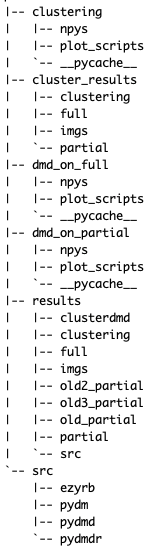
\includegraphics[width=2cm]{res/tree_brutto.png}
    \caption{\texttt{tree} della directory di un progetto.}\label{fig:tree}
\end{wrapfigure}
ambito dello stesso progetto) al fine di pervenire all'obiettivo preposto, eventualmente insieme all'aumentare del numero di parametri che controllano determinate caratteristiche degli stessi, rende la situazione ancora più caotica.  Il progetto si propone il compito di risolvere questo problema con una base di dati, al fine di evitare gerarchie di cartelle con cui risulta difficoltoso lavorare a lungo termine (come quella in Figura \ref{fig:tree}).

Il progetto sarà modelizzato nella forma di un algoritmo, che prende in input un dataset ed una n-upla di parametri, viene eseguito su un hardware di qualche tipo, e restituisce un dataset che contiene il risultato dell'esperimento. Saranno fatte alcune ipotesi che, pur restringendo il campo di applicazione, sono facilmente generalizzabili e servono solamente a rendere più concreta l'esposizione.

\section{Ipotesi}
\label{sec:ipotesi}
Si supporrà che sui cluster presi in considerazione sia installato il workload manager \texttt{Slurm}. Inoltre l'utente incarnato dal wrapper che ingloba la base di dati deve avere i diritti di lettura e scrittura ovunque sia necessario, su tutte le macchine registrate nella tabella \fbox{Hardware}.

Gli algoritmi saranno implementati in Python (un linguaggio molto usato in ambito scientifico) ed accetteranno parametri posizionali di tipo intero corrispondenti ad indici di liste definite negli stessi algoritmi. Queste saranno definite all'interno degli algoritmi in questo modo:

\verb|pod_ranks = [1-1.e-3, 1-1.e-6, 1-1.e-9, 1-1.e-12, -1]|

Ad esempio, lanciando uno script con ``\texttt{python3 script.py 2}'' si eseguirà l'algoritmo prendendo come primo parametro il terzo valore della lista \texttt{pod\_ranks}. Questa supposizione ci consente di delegare all'utente la definizione di tipi di input fantasiosi e potenzialmente non supportati dal DBMS.

Si supporrà che le implementazioni degli algoritmi siano disponibili istantaneamente su tutte le macchine. Trattandosi solitamente di script solitamente leggeri perchè privi di UI, la sincronizzazione tra dispositivi risulta molto semplice e possiamo ignorarla.

Su tutte le macchine sarà installato di default il package manager \href{https://pypi.org/project/pip/}{pip}, uno dei più popolari per l'installazione di librerie Python.

Saranno supportati solamente esperimenti deterministici: ci aspettiamo che l'esecuzione di uno stesso algoritmo sullo stesso hardware, con la stessa tupla di parametri e lo stesso dataset in input restituisca lo stesso risultato (con eventualmente qualche fluttuazione di lieve importanza nella durata dell'esperimento).

Infine si suppone che i vincoli riguardanti la versione di una libreria siano solamente di tipo $\geq$. In altre parole, se un'istanza di \fbox{Algorithm} richiede l'installazione della \fbox{Library} \{\texttt{'Name':'numpy', 'Version':'1.20'}\}, saranno considerate valide anche le versioni \texttt{1.20.1}, \texttt{1.20.2}, etc. Si potrebbero presentare casi in cui non vi è più \emph{backward compatibility} oltre una certa versione, ma si considera consigliabile in questo caso sistemare l'implementazione per utilizzare la nuova interfaccia.

\section{Schema concettuale}
% ammettiamo che una Run non ritorni un Data perchè potrebbe dare errore
\begin{figure}[H]
    \makebox[\textwidth][c]{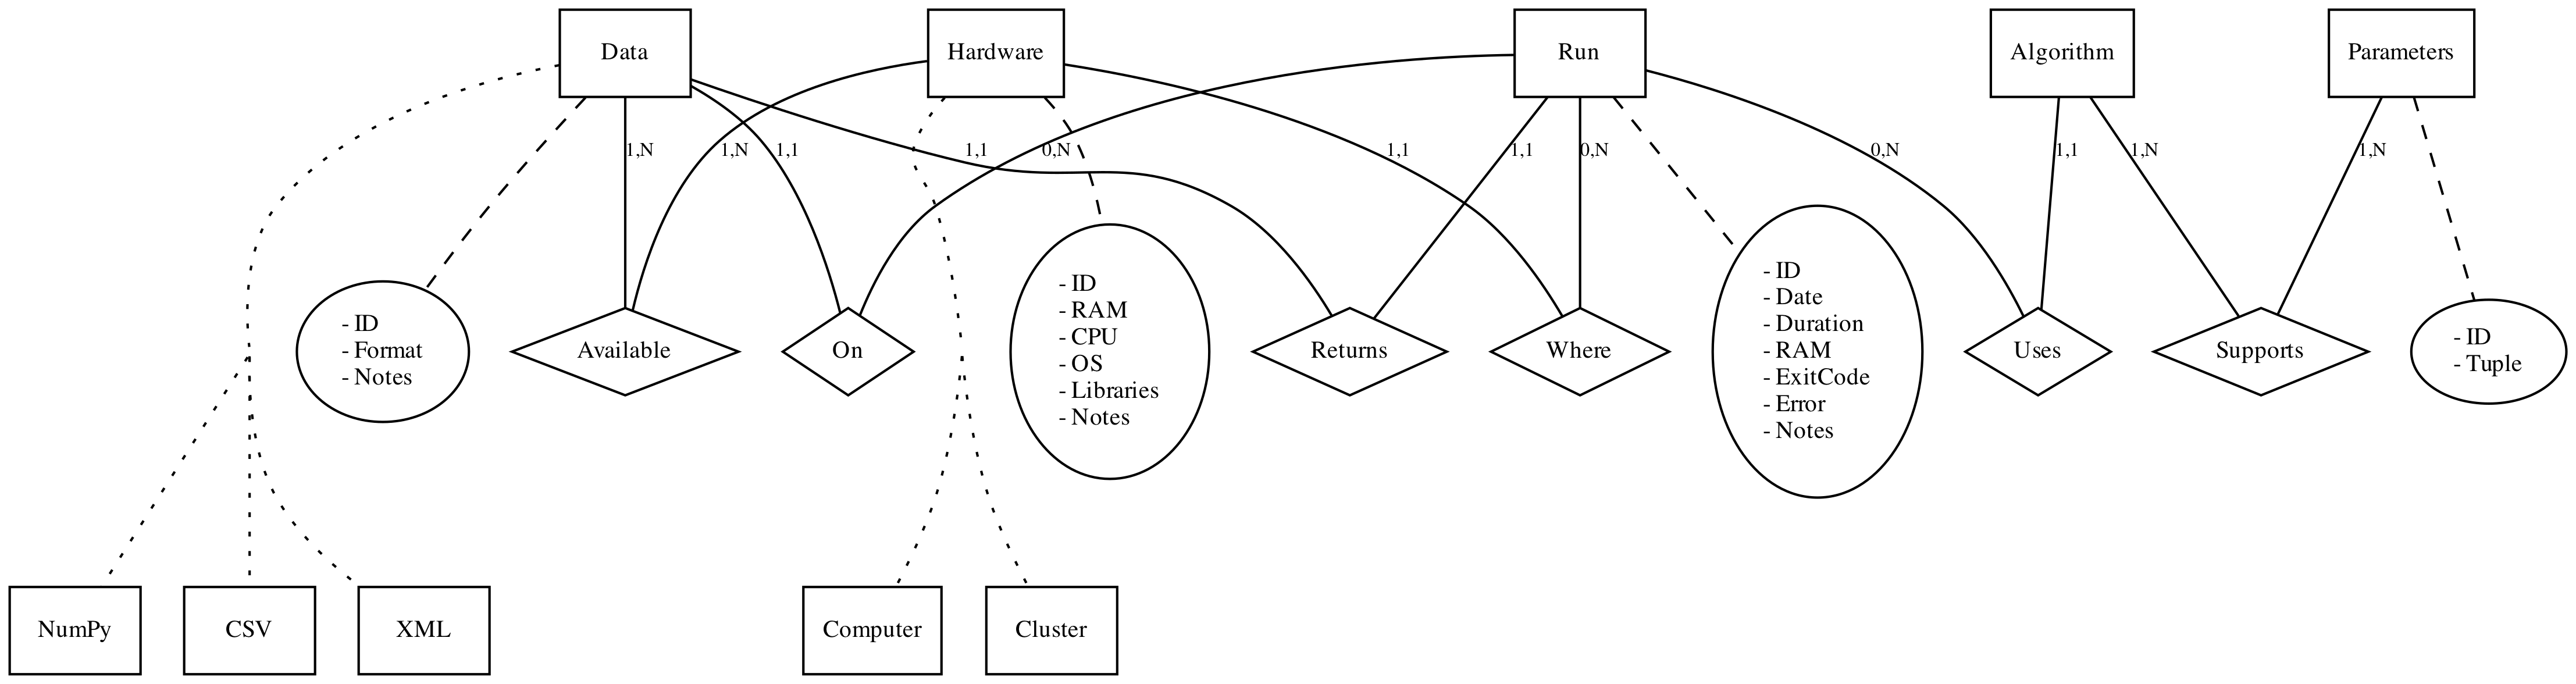
\includegraphics[width=1.6\textwidth]{res/schema_concettuale.png}}
    \caption{Schema concettuale del progetto.}
\end{figure}
Viene fornita una descrizione sintetica delle entità, delle relazioni e degli attributi.
\begin{itemize}
    \item \fbox{Algorithm}: L'implementazione di un particolare metodo sperimentato, nella pratica le istanze di \fbox{Algorithm} possono differire di poco, ma non tenteremo alcuna associazione visto che in diversi ambiti un piccolo cambiamento porta a risultati molto diversi. Per questo motivo diverse versioni di uno stesso algoritmo sono considerate come algoritmi differenti.

    Ogni algoritmo viene implementato in una specifica \emph{branch}, lo script necessario per il lancio deve trovarsi in un percorso ben specificato dalla root del repository (ad esempio \texttt{src/launchscript.py}). Le entità di tipo \fbox{Algorithm} inoltre sono identificate dal codice corrispondente ad una \emph{commit}.

    E' possibile utilizzare la relazione \emph{Fixes} tra due istanze di \fbox{Algorithm} per evidenziare il fatto che uno è una versione successiva dell'altro. Inoltre la relazione \emph{Needs} consente di specificare eventuali librerie non standard (sotto forma di istanze di \fbox{Library}) necessarie per l'esecuzione dell'algoritmo.
    \item \fbox{Parameters}: Ogni riga contiene una tupla univoca di interi che rappresenta una possibile lista di parametri di un algoritmo, come specificato nella Sezione \ref{sec:ipotesi}. Non tutte le tuple di parametri sono supportate da tutti gli algoritmi, dato che alcuni possono richiedere un numero inferiore o superiore di parametri a seconda del metodo che implementano. Per questo motivo è stata aggiunta la relazione \emph{Supports}.
    \item \fbox{Library}: Una libreria non standard, identificata univocamente da nome e versione. Si supporrà che la disponibilità di una libreria su una macchina implichi la sua presenza all'interno della variabile di sistema \texttt{PATH}, il che consente di evitare di specificare un percorso per raggiungere i file necessari.

    Una libreria può dipendere da altre librerie, ovvero volendo utilizzare una libreria $X$ che dipende dalle librerie $[A,B,C]$ è necessario avere installate $[A,B,C]$ sulla macchina su cui si intende eseguire l'esperimento. La relazione \emph{Depends} modelizza questo requisito.
    \item \fbox{Data}: Dataset di input, oppure output di una particolare \fbox{Run} caratterizzata da un \emph{Name}. Prendiamo in considerazione diversi formati: NumPy, XML, CSV. Ognuno richiede da parte dell'utilizzatore (che può essere un utente oppure un'istanza di \fbox{Algorithm}) metodi differenti per l'apertura.

    Essendo i dataset in generale considerevolmente pesanti, non possiamo supporre che ciascuno sia disponibile istantaneamente su tutte le macchine. Per questa ragione è stata introdotta la relazione \emph{Available}, che lega coppie di dataset a macchine su cui sono disponibili senza operazioni intermedie (che possono richiedere del tempo).
    \item \fbox{Run}: Il risultato di un esperimento con un ben specificato \fbox{Algorithm} (tramite la relazione \emph{Uses}), su un \fbox{Hardware} specifico (relazione \emph{Where}), applicato ad un'istanza di \fbox{Data} in input (relazione \emph{On}), con una precisa tupla di parametri (relazione \emph{With}).

    L'attributo \emph{Date} registra la data di esecuzione dell'esperimento (nel caso di esperimenti lunghi, la data di inizio), \emph{Duration} la durata in secondi, \emph{RAM} la memoria complessiva utilizzata, \emph{ExitCode} il codice restituito dallo script (che può essere utilizzato per verificare l'eventuale occorrenza di errori), \emph{Error} una stringa esplicativa dell'eventuale errore occorso.
    \item \fbox{Hardware}: Rappresenta una macchina a disposizione dell'organizzazione che conduce l'esperimento. Gli attributi \emph{RAM, CPU, OS} consentono di memorizzare le specifiche del dispositivo. Le istanze di \fbox{Hardware} possono essere computer singoli o cluster, ed in quest'ultimo caso avremo un attributo in più, \emph{Nodes}, che immagazzina il numero di nodi disponibili sul cluster. E' possibile stabilire relazioni di tipo \emph{Has} tra istanze di \fbox{Hardware} e \fbox{Library} per specificare quali librerie sono installate su una particolare macchina.
\end{itemize}
Tutte le entità dispongono di un attributo \emph{Notes} per eventuali annotazioni relative ad una particolare istanza (per \fbox{Algorithm} un commento sulla metodologia utilizzata dall'algoritmo, per \fbox{Hardware} eventuali problemi ricorrenti con quella particolare macchina, ad esempio).

\section{Operazioni previste}
L'idea del progetto è automatizzare, eventualmente con un'interfaccia di qualche tipo oltre alla base di dati, l'intera pipeline di comandi che porta dalla situazione in cui si dispone di dataset, hardware, algoritmo e parametri, a quella in cui sono stati generati i risultati dell'esperimento corrispondente a questa 4-upla. Nel mezzo vengono dunque inglobati i seguenti compiti:
\begin{itemize}
    \item Verifica della realizzabilità di un esperimento (Sulla macchina è disponibile il dataset di input su cui si intende eseguire l'algoritmo? Sono installate le librerie richieste dall'algoritmo, e tutte le librerie da cui dipendono?)
    \item Generazione del comando per lanciare lo script in cui consiste l'esperimento, che tiene conto dei parametri e della piattaforma (nel caso di un cluster il comando sarà del tipo \texttt{sbatch ...});
    \item Scrittura dei risultati in una directory con nome dipendente da ognuno degli elementi che caratterizzano l'esperimento (algoritmo usato, parametri, hardware, dataset).
    \item Comunicazione all'utente della posizione della directory corrispondente ad una particolare n-upla algoritmo-hardware-dataset-parametri, o di una lista di directory nel caso in cui uno di questi elementi sia omesso.
\end{itemize}
Inoltre sarà necessario consentire la registrazione di nuovi algoritmi, hardware, dataset, parametri, librerie. Ci si aspetta inoltre che la base di dati generi la sequenza di comandi necessaria per l'installazione di una libreria su una macchina, e che sia possibile verificare se un'istanza di \fbox{Algorithm} può essere eseguita su un certo \fbox{Hardware}.

\section{Schema concettuale ristrutturato}
Sono state rimosse le generalizzazioni totali \fbox{Cluster} e \fbox{Computer} di \fbox{Hardware}, l'attributo \emph{Nodes} di \fbox{Cluster} è accorpato a \fbox{Hardware}, e vale coerentemente ``1'' se l'istanza è di tipo \fbox{Computer}.

Sono state rimosse le generalizzazioni parziali di \fbox{Data} in quanto la loro presenza non apportava un particolare contributo; sono state rimpiazzate dall'attributo \emph{Format}, che consente all'utente di conoscere in anticipo il formato del dataset per regolarsi di conseguenza sul metodo adeguato per aprirlo. Gli attributi \emph{Shape} e \emph{Dtype} di \emph{NumPy} possono essere ottenuti rapidamente una volta aperto il dataset (per evitare il costo del caricamento in RAM si può usare il comando \texttt{np.load(..., mmap\_mode='r')}).

E' stata rimossa l'entità \fbox{Parameters}, in quanto non aveva una particolare utilità ed anzi rendeva il tutto più complicato: possiamo considerare effettivamente differenti due istanze di uno stesso algoritmo con attributi \emph{Parameters} differenti, in quanto ci aspettiamo risultati del tutto indipendenti.

\begin{figure}[H]
    \makebox[\textwidth][c]{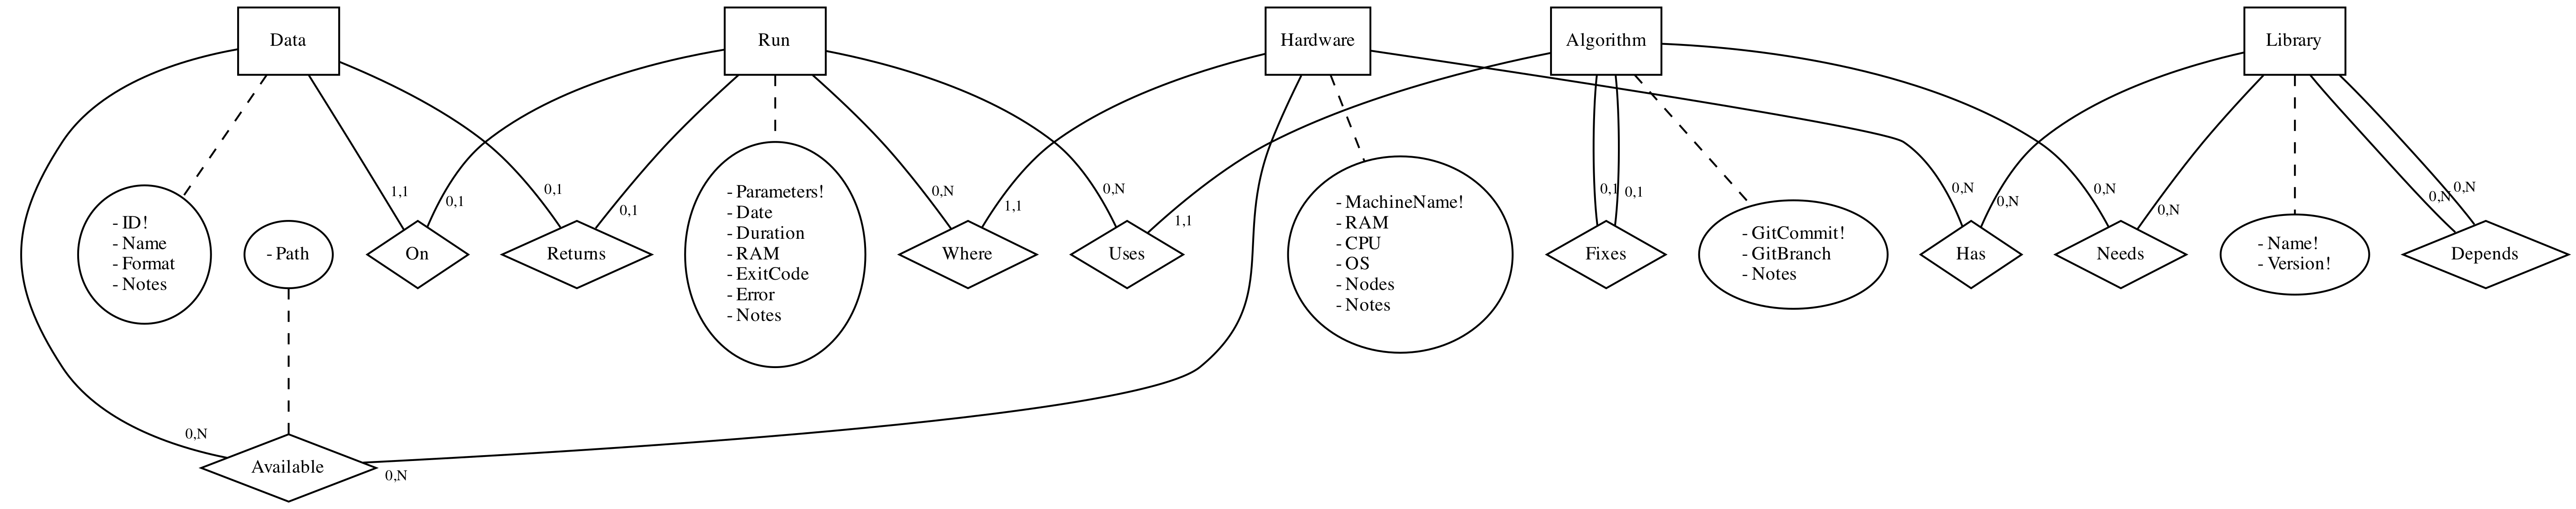
\includegraphics[width=1.6\textwidth]{res/schema_concettuale_ristrutturato.png}}
    \caption{Schema concettuale ristrutturato del progetto.}
\end{figure}

\section{Volumi}
Consideriamo la base di dati come uno strumento utilizzabile nell'ambito di un singolo progetto. Il paradigma è facilmente estensibile per la gestione simultanea di più progetti, è sufficiente aggiungere l'entità \fbox{Project} ed un attributo \emph{Project} alle entità \fbox{Run\vphantom{g}}, \fbox{Algorithm\vphantom{g}}, \fbox{Data\vphantom{g}}.
\begin{table}[H]
    \begin{minipage}[b]{.5\linewidth}
      \centering
      \begin{tabular}{||l l||}
        \hline
        Entità & Volume \\ [0.5ex]
        \hline\hline
        Data & $<5000 + 5$\\
        Hardware & $<5$\\
        Run & $<5000$\\
        Algorithm & $<1000$\\
        Library & $<200$\\
        \hline
       \end{tabular}
       \caption{Volumi delle entità.}
    \end{minipage}
    \begin{minipage}[b]{.5\linewidth}
      \centering
        \begin{tabular}{||l l||}
            \hline
            Relazione & Volume \\ [0.5ex]
            \hline\hline
            Available & $<25$\\
            On & $<5000$\\
            Returns & $<5000$\\
            Where & $<5000$\\
            Uses & $<5000$\\
            Needs & $<50000$\\
            Fixes & $<1000$\\
            Has & $<1000$\\
            Depends & $<<200*200$\\
            \hline
           \end{tabular}
           \caption{Volumi delle relazioni.}
    \end{minipage}
\end{table}

Ci si aspetta di avere all'incirca 5 dataset (tipo \fbox{Data}) in ingresso, un insieme ragionevole di esperimenti per considerare valido il metodo sperimentato. Abbiamo inoltre diversi algoritmi da testare  (tipo \fbox{Algorithm}): il numero alto di entità di questo tipo è dovuto al fatto che nuove versioni di uno stesso algoritmo (bugfix, nuove funzionalità, ...) sono considerate come entry differenti.

In genere testeremo un algoritmo con una combinazione di parametri ``veloce'' su un computer privato per eliminare immediatamente eventuali bug, per poi lanciare un pool di jobs su un cluster. Ogni esecuzione è rappresentata da un oggetto di tipo \fbox{Run}, e produce un output di tipo \fbox{Data}. L'esecuzione ``di test'' non è conteggiata perchè evidentemente influisce poco sul numero complessivo.

Il volume dell'entità \fbox{Library} è stato valutato come approssimazione del valore medio dell'output di \texttt{pip freeze | wc -l} su diversi computer, stimando il tutto per eccesso in quanto più versioni di una stessa libreria possono convivere nella base di dati (essendo installate su \fbox{Hardware} diversi).

\section{Schema logico}
\begin{table}[H]
    \makebox[\textwidth][c]{
    \begin{minipage}[t]{.5\linewidth}
      \centering
      \caption*{Library}
      \begin{tabular}{||l c l||}
        \hline
        Attributo & PK/FK & Tipo\\ [0.5ex]
        \hline\hline
        Name & PK & \\
        Version & PK & \\
        \hline
       \end{tabular}
    \end{minipage}
    \hfill
    \begin{minipage}[t]{.5\linewidth}
        \centering
        \caption*{Depends}
        \begin{tabular}{||l c l||}
          \hline
          Attributo & PK/FK & Tipo\\ [0.5ex]
          \hline\hline
          DependentName & PK,FK & \\
          DependentVersion & PK,FK & \\
          StandName & PK,FK & \\
          StandVersion & PK,FK & \\
          \hline
         \end{tabular}
      \end{minipage}
      \hfill
      \begin{minipage}[t]{.5\linewidth}
        \centering
        \caption*{Hardware}
        \begin{tabular}{||l c l||}
          \hline
          Attributo & PK/FK & Tipo\\ [0.5ex]
          \hline\hline
          MachineName & PK & \\
          RAM & & \\
          CPU & & \\
          OS & & \\
          Nodes & & \\
          Notes & & \\
          \hline
         \end{tabular}
      \end{minipage}
    }
\end{table}
\begin{table}[H]
    \makebox[\textwidth][c]{
    \begin{minipage}[t]{.5\linewidth}
      \centering
      \caption*{Has}
      \begin{tabular}{||l c l||}
        \hline
        Attributo & PK/FK & Tipo\\ [0.5ex]
        \hline\hline
        Hardware & PK/FK & \\
        LibraryName & PK/FK & \\
        LibraryVersion & PK/FK & \\
        \hline
       \end{tabular}
    \end{minipage}
    \hfill
    \begin{minipage}[t]{.5\linewidth}
        \centering
        \caption*{Algorithm}
        \begin{tabular}{||l c l||}
          \hline
          Attributo & PK/FK & Tipo\\ [0.5ex]
          \hline\hline
          GitCommit & PK & \\
          Parameters & PK & \\
          GitBranch & & \\
          Fixes & & \\
          Notes & & \\
          \hline
         \end{tabular}
      \end{minipage}
      \hfill
      \begin{minipage}[t]{.5\linewidth}
        \centering
        \caption*{Needs}
        \begin{tabular}{||l c l||}
          \hline
          Attributo & PK/FK & Tipo\\ [0.5ex]
          \hline\hline
          AlgorithmCommit & PK/FK & \\
          AlgorithmParameters & PK/FK & \\
          LibraryName & PK/FK & \\
          LibraryVersion & PK/FK & \\
          \hline
         \end{tabular}
      \end{minipage}
    }
\end{table}

\begin{table}[H]
    \makebox[\textwidth][c]{
    \begin{minipage}[t]{.5\linewidth}
      \centering
      \caption*{Data}
      \begin{tabular}{||l c l||}
        \hline
        Attributo & PK/FK & Tipo\\ [0.5ex]
        \hline\hline
        ID & PK & \\
        Name & & \\
        Format & & \\
        Notes & & \\
        \hline
       \end{tabular}
    \end{minipage}
    \hfill
    \begin{minipage}[t]{.5\linewidth}
        \centering
        \caption*{Available}
        \begin{tabular}{||l c l||}
          \hline
          Attributo & PK/FK & Tipo\\ [0.5ex]
          \hline\hline
          Hardware & PK/FK & \\
          Data & PK/FK & \\
          Path & & \\
          \hline
         \end{tabular}
      \end{minipage}
      \hfill
      \begin{minipage}[t]{.5\linewidth}
        \centering
        \caption*{Run}
        \begin{tabular}{||l c l||}
          \hline
          Attributo & PK/FK & Tipo\\ [0.5ex]
          \hline\hline
          Algorithm & PK/FK & \\
          InputData & PK/FK & \\
          Hardware & PK/FK & \\
          OutputData & FK & \\
          Date & & \\
          Duration & & \\
          RAM & & \\
          ExitCode & & \\
          Error & & \\
          Notes & & \\
          \hline
         \end{tabular}
      \end{minipage}
    }
\end{table}

\section{Note}
Si potrebbe pensare che lasciare nella tabella \fbox{Library} un numero indefinito di versioni di una stessa libreria sia dannoso in termini di spazio: sarebbe sufficiente mantenere solo le librerie referenziate dall'ultima versione di un algoritmo. Il motivo per cui non si è scelto di inserire un \emph{check} per cancellare in modo autonomo dalla tabella librerie che siamo certi non saranno più usate in una \fbox{Run} è che si intende mantenere un database di snapshot: poter ricostruire nel dettaglio quali librerie ed in quale versione erano presenti sulla macchina è fondamentale per risolvere bug o verificare risultati inattesi. E' anche il motivo per cui si consiglia di specificare la versione delle librerie nel file \texttt{requirements.txt}. Per glis stessi motivi consentiamo la convivenza di più versioni di una libreria su uno stesso \fbox{Hardware} (resa possibile da utility come \texttt{pipenv}).

Questo documento è stato realizzato con \LaTeX. Gli schemi sono stati realizzati in Python utilizzando le librerie \href{https://networkx.org/documentation/stable/index.html}{\emph{NetworkX}} e \emph{(Py)\href{http://www.graphviz.org/}{Graphviz}}, ed il VCS \emph{git}. Il codice sorgente per schemi e documento è disponibile nel repository GitHub \href{https://github.com/fAndreuzzi/BDD}{fAndreuzzi/BDD}.

L'idea per questo progetto è stata ispirata dalla collera conseguente alla necessità di dover eseguire da zero un pool di 400 \emph{jobs} sul cluster HPC della SISSA perchè i risultati corrispondenti erano stati sovrascritti da un altro esperimento con un algoritmo diverso ma parametri identici.

\end{document}
